% !TEX root = stack-thresh.tex

%============================================================================================
\section{Numerical results}
\label{sec:numerical}

In this section, we illustrate the results of Sections~\ref{sec:cost} and~\ref{sec:threshold} by numerically simulating the NCF strategy and computing its cost on an example network.
We generated a network with $\NLinks = 5$ links, and arbitrary latency functions, shown in Fig.~\ref{fig:num_latencies}. 

\begin{figure}[h]
\centering
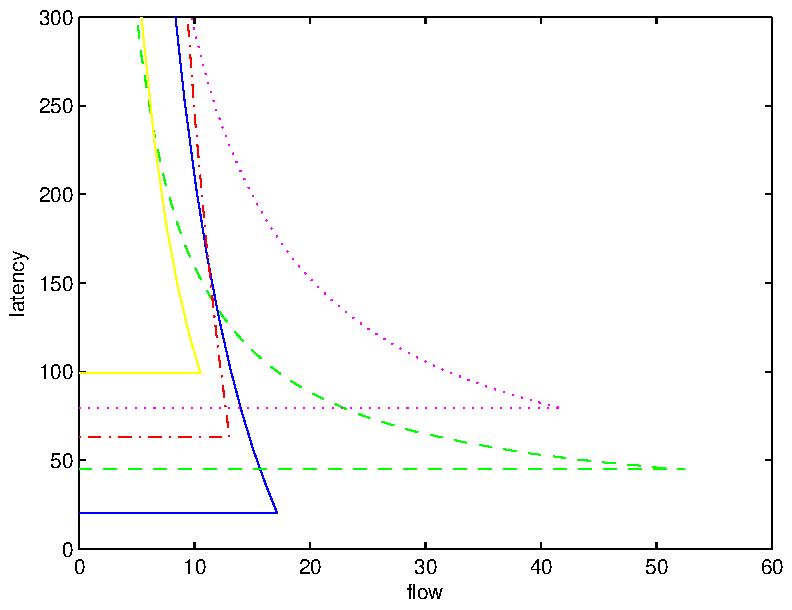
\includegraphics[width = 2.5in]{figures/latencies}
\caption{Latency functions for the example network.}
\label{fig:num_latencies}
\end{figure}

The optimal Stackelberg cost is computed for ${ \demand \in [0, \demandMax{\NLinks}] }$ and $\compRate \in [0,1]$. The results are shown in Fig.~\ref{fig:num_cost}. For a fixed demand, the optimal cost is a piecewise constant function of $\compRate$ (Fig.~\ref{fig:num_cost_2}). This also illustrates the intervals $\{I_j\}_{1 \leq j \leq j_0}$ discussed in the previous section. In this example, we have $\demandMax{1} < \demandMax{2} \leq \demandMax{3} < \demandMax{4} \leq \demandMax{5}$, therefore the links that achieve a strict increase in the capacity are $k_1 = 1$, $k_2 = 2$ and $k_3 = 4$.

\begin{figure}[h]
\centering
\begin{subfigure}[b]{3.3in}
\centering
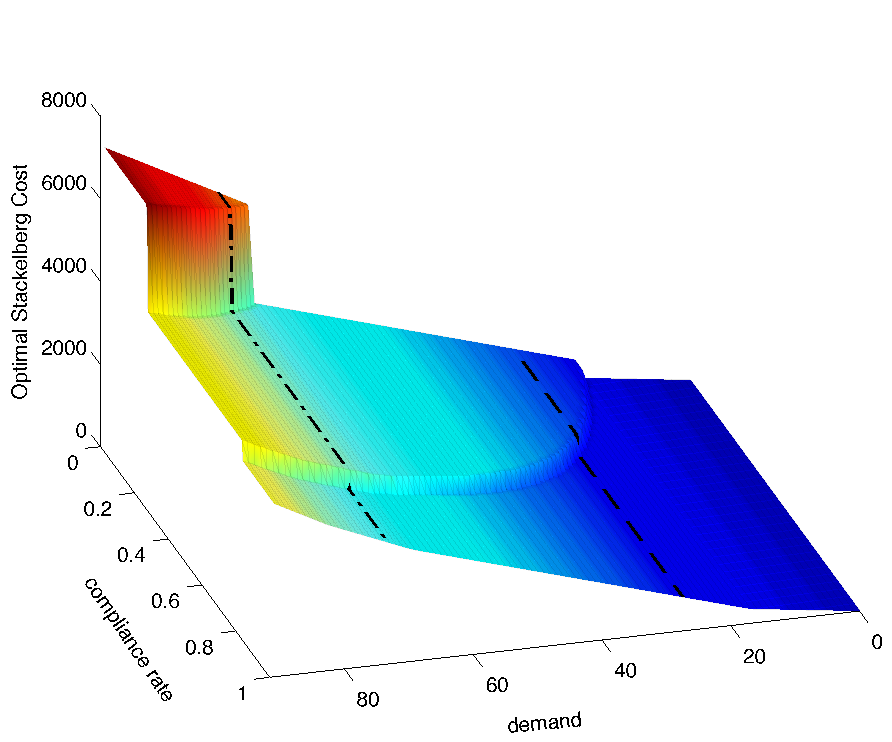
\includegraphics[width=2.8in]{figures/cost_surface}
\caption{Optimal Stackelberg cost as a function of $\demand$ and~$\compRate$. Iso-$\demand$ lines are plotted for $\demand = 0.3 \ \demandMax{\NLinks}$ (dashed) and ${ \demand = 0.8 \ \demandMax{\NLinks} }$ (dot-dashed).}
\label{fig:num_cost_1}
\end{subfigure}

\begin{subfigure}[b]{3.3in}
\vspace{10pt}
\centering
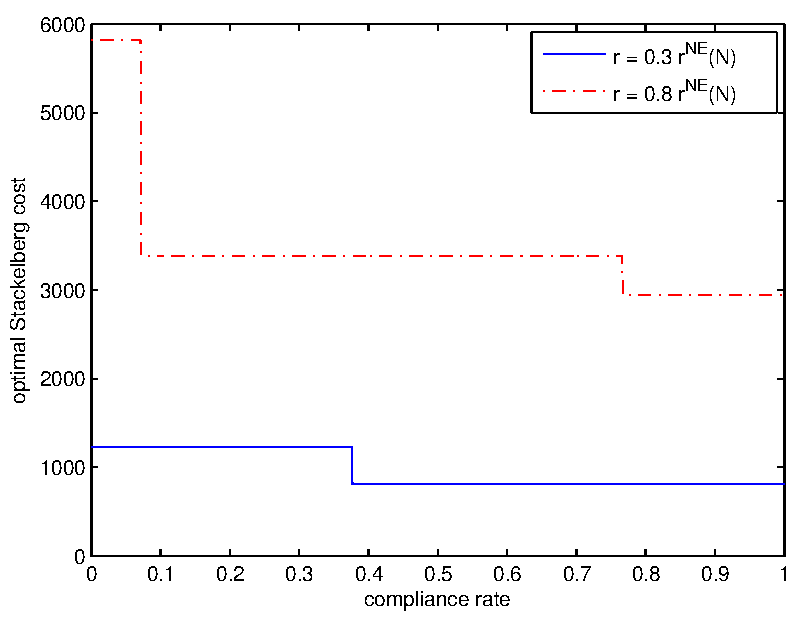
\includegraphics[width=2.6in]{figures/cost}
\caption{$C_{\textup{NCF}}(\compRate)$: optimal Stackelberg cost for a fixed demand $\demand$. The cost is a non-increasing, piecewise constant function of~$\compRate$. When the demand is ${ \demand = 0.8 \ \demandMax{\NLinks} }$, we have $j_0 = 3$, therefore we have two discontinuities, at $1 - \frac{\demandMax{k_1}}{\demand}$ and $1 - \frac{\demandMax{k_2}}{\demand}$.}
\label{fig:num_cost_2}
\end{subfigure}

\caption{Optimal Stackelberg cost.}
\label{fig:num_cost}
\end{figure}


Finally, we numerically compute and plot the Stackelberg threshold for different values of the demand. The results, shown in Fig.~\ref{fig:num_stack_thresh}, match the analytical expression given in Proposition~\ref{prop:thresh}. We observe that for low values of demand ($\demand < \demandMax{1}$), the social optimum and the Nash equilibrium ($\compRate = 0$) are identical, therefore Stackelberg routing cannot strictly improve the cost. For $\demand > \demandMax{1}$, we observe two branches: the first one corresponds to the range of demands $\demand \in ]\demandMax{1}, \demandMax{2}]$, for which the Stackelberg threshold is given by $1-\frac{\demandMax{k_1}}{\demand}$ ($j_0 = 2$, i.e. $k(0) = k_2 = 2$). The second one corresponds to the range of demands $]\demandMax{2}, \demandMax{4}]$, for which the Stackelberg threshold is given by $1-\frac{\demandMax{k_2}}{\demand}$ ($j_0 = 3$, i.e. $k(0) = k_3 = 4$).


\begin{figure}[h]
\centering
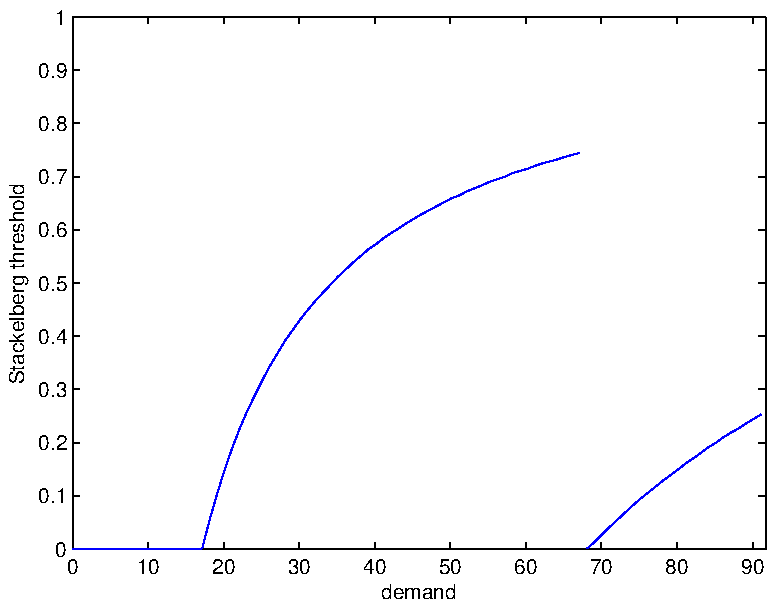
\includegraphics[width = 2.6in]{figures/threshold}
\caption{Stackelberg threshold for increasing values of demand.}
\label{fig:num_stack_thresh}
\end{figure}


